\documentclass{cmc}

\begin{document}

\pagestyle{fancy}
\lhead{\textit{\textbf{Computational Motor Control, Spring 2022} \\
    Python exercise, Lab 1, NOT GRADED}} \rhead{Student \\ Names}

\section*{Student names: \ldots (please update)}

\textit{Instructions: Update this file (or recreate a similar one, e.g.\ in
  Word) to prepare your answers to the questions. Feel free to add text,
  equations and figures as needed. Hand-written notes, e.g.\ for the development
  of equations, can also be included e.g.\ as pictures (from your cell phone or
  from a scanner).  \textbf{This lab is not graded. However, the lab exercises
    are meant as a way to familiarise with dynamical systems and to study them
    using Python to prepare you for the final project.} This file does not need
  to be submitted and is provided for your own benefit. The graded exercises
  will have a similar format.}

\textit{In this exercise, you will familiarise with ODE integration methods, how
  to plot results and study integration error. The file \fileref{lab\#.py} is
  provided to run all exercises in Python. Each \fileref{exercise\#.py} can be
  run to run an exercise individually. The list of exercises and their
  dependencies are shown in Figure~\ref{fig:files}. When a file is run, message
  logs will be printed to indicate information such as what is currently being
  run and and what is left to be implemented. All warning messages are only
  present to guide you in the implementation, and can be deleted whenever the
  corresponding code has been implemented correctly.}

\begin{figure}[ht]
  \centering 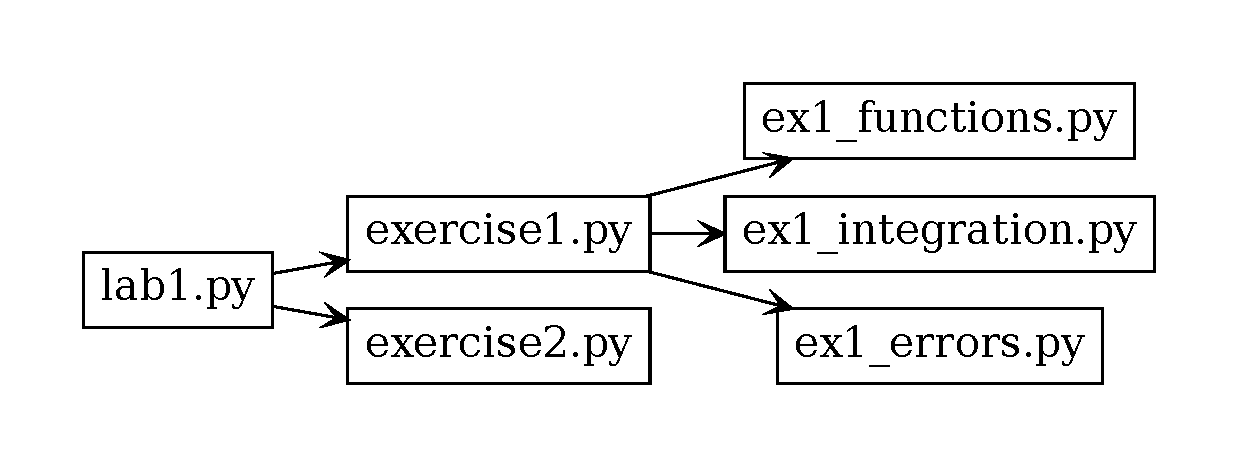
\includegraphics[width=0.5\textwidth]{figures/files}
  \caption{\label{fig:files} Exercise files dependencies. In this lab, you will
    be modifying \fileref{exercise1.py}, \fileref{ex1\_functions.py},
    \fileref{ex1\_integration.py},\fileref{ex1\_errors.py} and
    \fileref{exercise2.py}. It is recommended to check out
    \fileref{exercise1.py} before looking into the other \fileref{ex1\_*.py}
    files.}
\end{figure}


\section*{Running the exercises}
\label{sec:inst-depend}

In order to run the exercises for Lab1 make sure to update your git packages.
You can do this by executing the following commands:

\begin{itemize}
\item Open the terminal
\item Navigate to the exercise repository (Make sure you are in the
  root of the folder)
\item Execute,
  \begin{itemize}
  \item \lstinline[columns=fixed]{$ git pull}
  \item \lstinline[columns=fixed]{$ pip install -r requirements.txt}
  \end{itemize}
\end{itemize}


\corr{NOTE : } Make sure to activate your virtualenv before running the exercise
codes.

\newpage
\section*{Question 1: Numerical integration}

\subsection*{1.a Compute the analytical solution x(t) % chktex 36
  for the following linear dynamical system. Provide here the calculation steps,
  then implement the solution in
  \fileref{ex1\_fun\-ctions.py::ana\-lytic\_fun\-ction()} % chktex 36
  and run \fileref{exercise1.py} to plot the result.}

\begin{equation}
  \label{eq:ode-1}
  \dot{x} = 2 \cdot (5 - x), \quad x(t=0)=1
\end{equation}


\vspace{0.3\textheight}


\newpage
\subsection*{1.b In some cases, an ODE system may not have an analytical
  solution or it may be difficult to compute. Implement Euler integration in
  \fileref{ex1\_integ\-ration.py::eu\-ler\_int\-eg\-rate()}, % chktex 36
  then run \fileref{exer\-cise1.py} again to compare the solution of
  \texttt{eu\-ler\_integr\-ate()} (with 0.2 timestep) % chktex 36
  to the analytical solution obtained previously and include a figure of the
  result here. Make sure to also implement
  \fileref{ex1\_fun\-ctions.py::fun\-ction()} % chktex 36
  so that the code may be run correctly. \\ As a code template, check out
  \fileref{ex1\_integ\-ration.py::eu\-ler\_exam\-ple()}.}



\vspace{0.3\textheight}



\clearpage

\subsection*{1.c Various efficient libraries are available to facilitate ODE
  integration. Compare the Euler method with Lsoda
  (\fileref{ex1\_integ\-ration.py::ode\_intg\-rate()}) % chktex 36
  and Runge-Kutta 4th order
  (\fileref{ex1\_integ\-ration.py::ode\_intg\-rate\_rk()}) % chktex 36
  integration methods by completing the corresponding functions using the scipy
  library in Python. See \fileref{exer\-cise1.py::exer\-cise1()} % chktex 36
  for the function calls. Provide the error values (there are multiple ways you
  could do this, choose an appropriate method and explain why), number of time
  steps, and include a figure comparing the integration methods. }



\vspace{0.3\textheight}



\clearpage

\subsection*{1.d As mentioned in the course, the comparison of question 1.c is
  not fair for the Euler method.  Briefly say why. Choose another number of time
  steps for the Euler method that is fairer when compared to
  Runge-Kutta. Provide the error values, number of time steps, and include a
  figure comparing the two integration methods. Briefly discuss which
  integration method is best.}



\vspace{0.3\textheight}



\clearpage

\subsection*{1.e Test the role of the step size by plotting the integration
  error as a function of step size. You can use
  \fileref{ex1\_errors.py::com\-pute\_err\-or()} % chktex 36
  to do this by completing the code in
  \fileref{ex1\_errors.py::error()}. % chktex 36
  How accurate is the solution compared to the analytical solution for different
  step sizes?  Include here a graph showing the error against the step
  size. Explain which error measure you used (there are several options)}



\vspace{0.3\textheight}



\clearpage

\section*{Question 2: Stability analysis}

\subsection*{2.a Find the fixed points of the following linear dynamical system,
  and analyze their stability (briefly describe the calculation steps).}

\begin{equation}
  \label{eq:system}
  \dot{x} = A x,
  \qquad
  A =
  \begin{pmatrix}
    \begin{array}{rr}
      1 & 4 \\
      -4 & -2
    \end{array}
  \end{pmatrix}
\end{equation}



\vspace{0.3\textheight}



\clearpage

\subsection*{2.b Perform numerical integration from different initial conditions
  to verify the stability properties. See \fileref{exercise2.py::exercise2()}
  for implementation. Include some figures with these different time evolutions
  and their corresponding phase portrait and explain their roles.}


\clearpage

\subsection*{2.c Change one value in matrix A such that the time evolution
  becomes periodic for some initial conditions. Say which value and include a
  time evolution figure.}



\vspace{0.3\textheight}



\clearpage

\subsection*{2.d Compute the eigenvalues and eigenvectors of the following system.
What can you say about the stability of its fixed point? What is the meaning of its
eigenvectors? Try to plot the flow of the system to get an intuition of its behavior.}

  \begin{equation}
    \label{eq:saddle-system}
    \dot{x} = A x,
    \qquad
    A =
    \begin{pmatrix}
      \begin{array}{rr}
        1 & 1 \\
        4 & -2
      \end{array}
    \end{pmatrix}
  \end{equation}


\vspace{0.3\textheight}



\end{document}